%!TEX root = ../template.tex
%%%%%%%%%%%%%%%%%%%%%%%%%%%%%%%%%%%%%%%%%%%%%%%%%%%%%%%%%%%%%%%%%%%%
%% chapter2.tex
%% NOVA thesis document file
%%
%% Chapter with the template manual
%%%%%%%%%%%%%%%%%%%%%%%%%%%%%%%%%%%%%%%%%%%%%%%%%%%%%%%%%%%%%%%%%%%%

\typeout{NT FILE chapter2.tex}%

\chapter{Low dimensional representations of locomotor parameters distinguish cerebellar mutants}
\label{cha:lda}
\glsresetall

\section{Abstract}
\section{Introduction}

% \section{Behavioral quantification}
\section{Results}
\subsection{Interlimb parameters separate cerebellar mutants and controls}

\begin{figure}
    \centering
    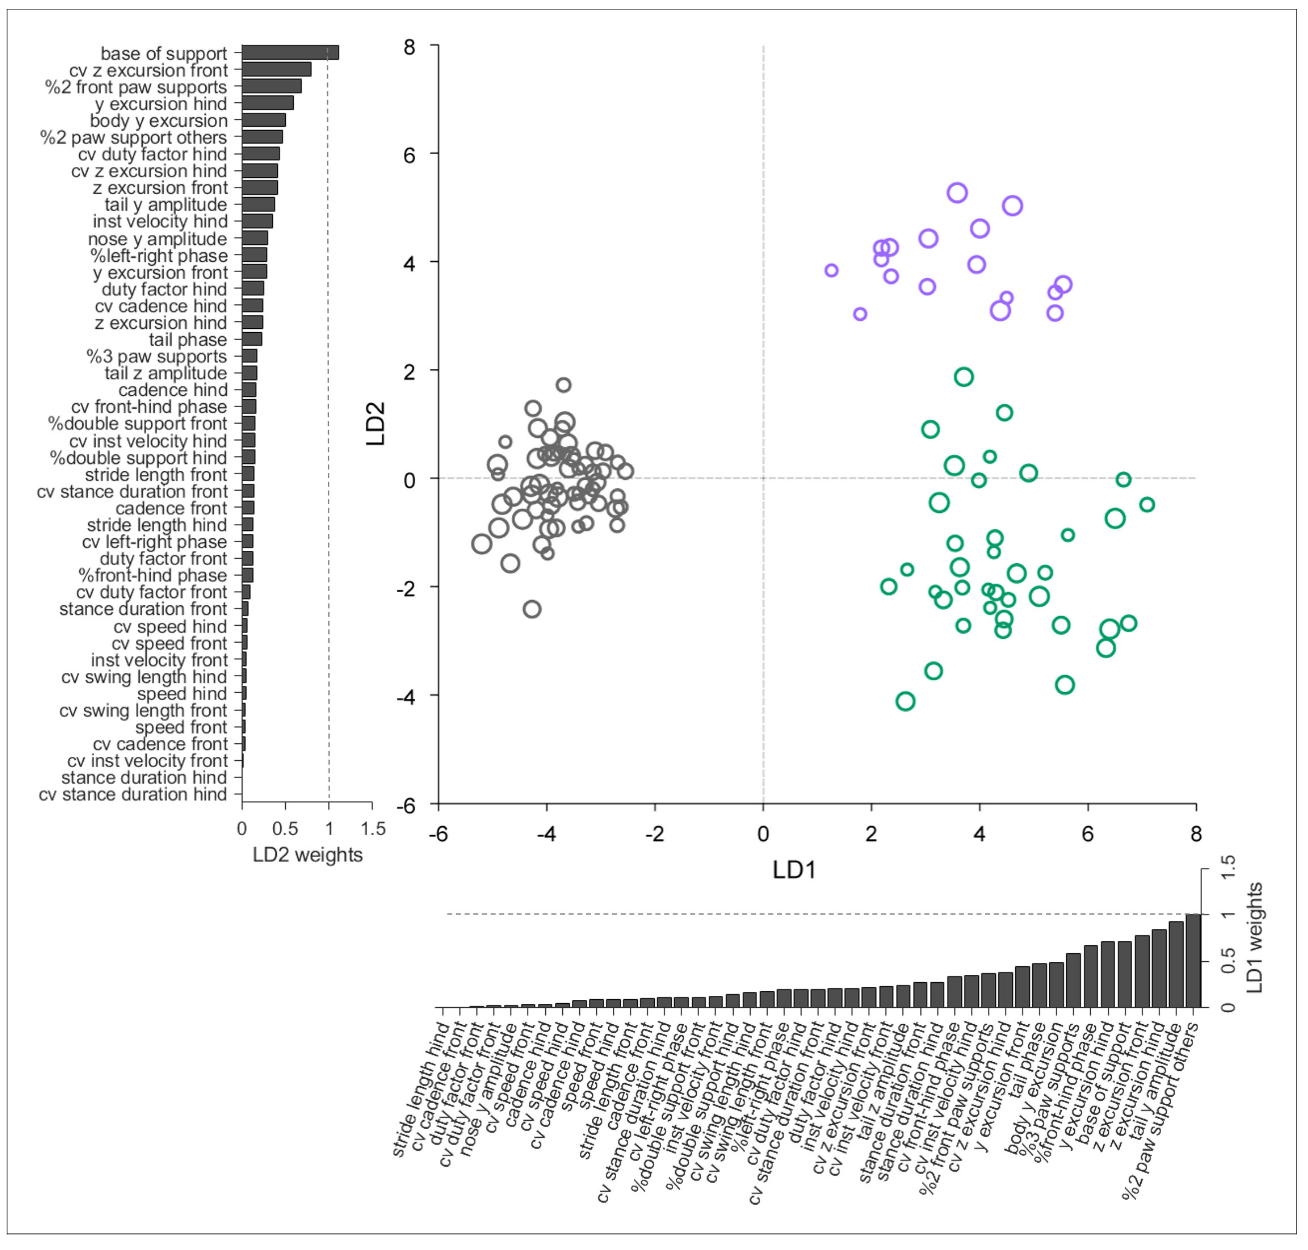
\includegraphics[width=1\linewidth]{Chapters//Figures//chapter2/LDA.png}
    \caption{Linear discriminant analysis of locomotor kinematics reveals two axes, which separate ataxic mutants from controls (LD1) and from each other (LD2). Each dot represents a single animal walking at a particular speed. Faster speeds are shown with larger marker sizes. Speeds ranged from 0.05 to 0.35 m/s and were binned with a bin width of 0.05 m/s. Size-matched controls are in grey (N = 11 for all speed bins; n = ~ 3288), reeler in green (N = 7 for 0.05–0.15 m/s; N = 6 for 0.25–0.35 m/s; n = ~ 2387), and pcd in purple (N = 3 for all speed bins except 0.25–0.30 m/s N = 2; n = ~ 3066). The bars along each axis are ranked by the contribution scores (LD coefficients) of each variable to that axis (larger bars indicate higher contributions). Features contributing strongly to LD1 (which accounts for 84\% of the total between-group variance) include interlimb and whole-body coordination, as well as off-axis paw trajectories. For LD2 (which accounts for 16\% of the between-group variance), they also include variability, front paw supports, and relative phasing of tail/nose movements.\\ Reproduced from Machado et al. 2020 \cite{machado_shared_2020}.}
    \label{fig:LDA}
\end{figure}

\subsection{Low dimensional representation of kinematics}

\begin{figure}
    \centering
    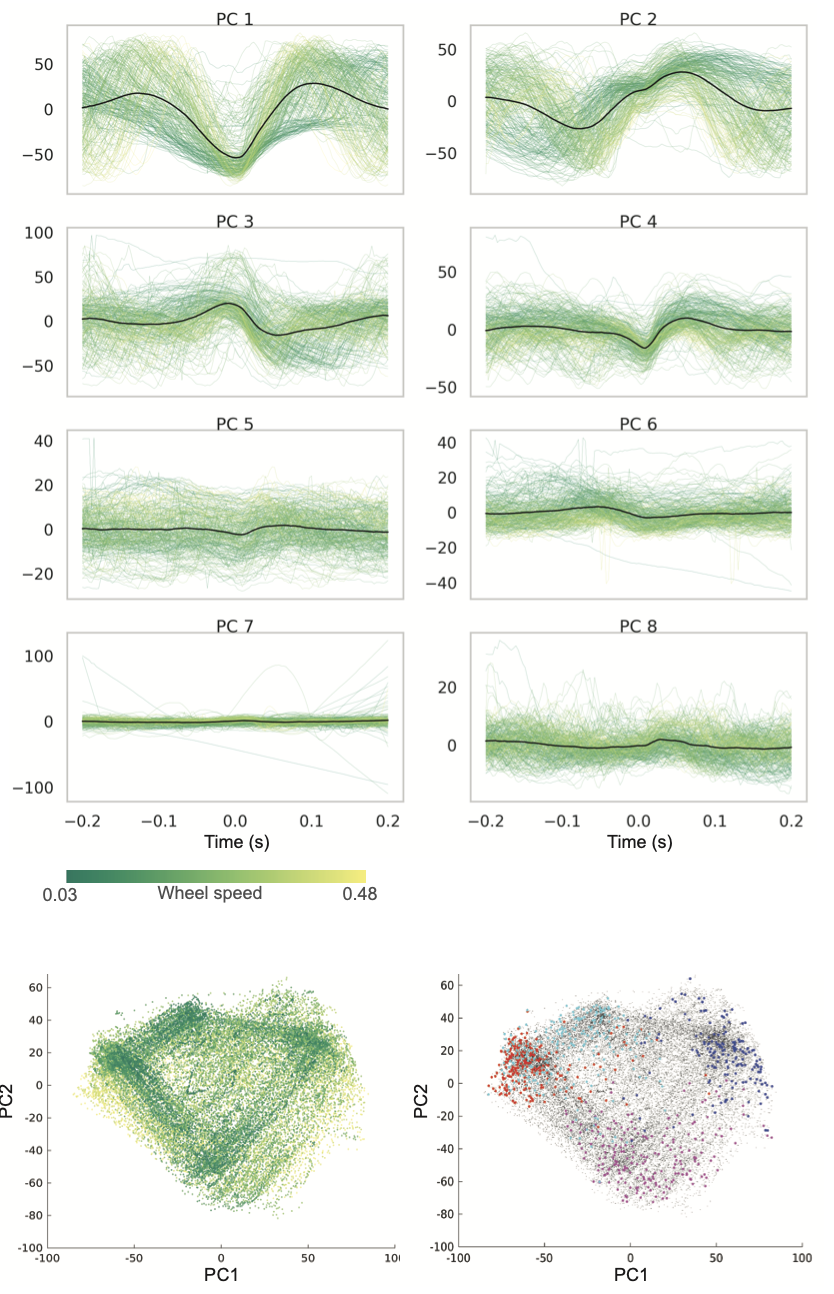
\includegraphics[width=1\linewidth]{Chapters//Figures//chapter2/behavioral_PCA.png}
    \caption{Principal component projections of instamntaneous paw positions}
    \label{fig:behav-pca}
\end{figure}

\section{Discussion}
\section{Methods}
\subsection{Animal models of cerebellar ataxia: PCD and Reeler mutants} % (fold)
\subsection{Behavior tracking in Locomouse}
\subsection{Quantification of locomotor parameters} % (fold)
\subsection{Linear discriminant analysis} % (fold)

% \section{Locomotion lies on a cyclical manifold in low dimension}
% \subsection{Principal component analysis of instantaneous body positions} % (fold)
% \subsection{Low dimensional representations of locomotion} % (fold)
% \subsection{Encoding of locomotor phase and speed} % (fold)

% \section{Exploring locomotor cycle stereotipy}
